\section{Pre-selection kinematic variables} \label{app:presel_plots}

Figures~\ref{fig:input_vars_3l_xsec}, \ref{fig:input_vars_2lss_xsec_mumu} and~\ref{fig:input_vars_2lss_xsec_emu} show the distributions of some relevant kinematic variables, normalized to the cross section of th\
e respective processes and to the integrated luminosity.
\newpage
\begin{figure} [!h]
  \centering
  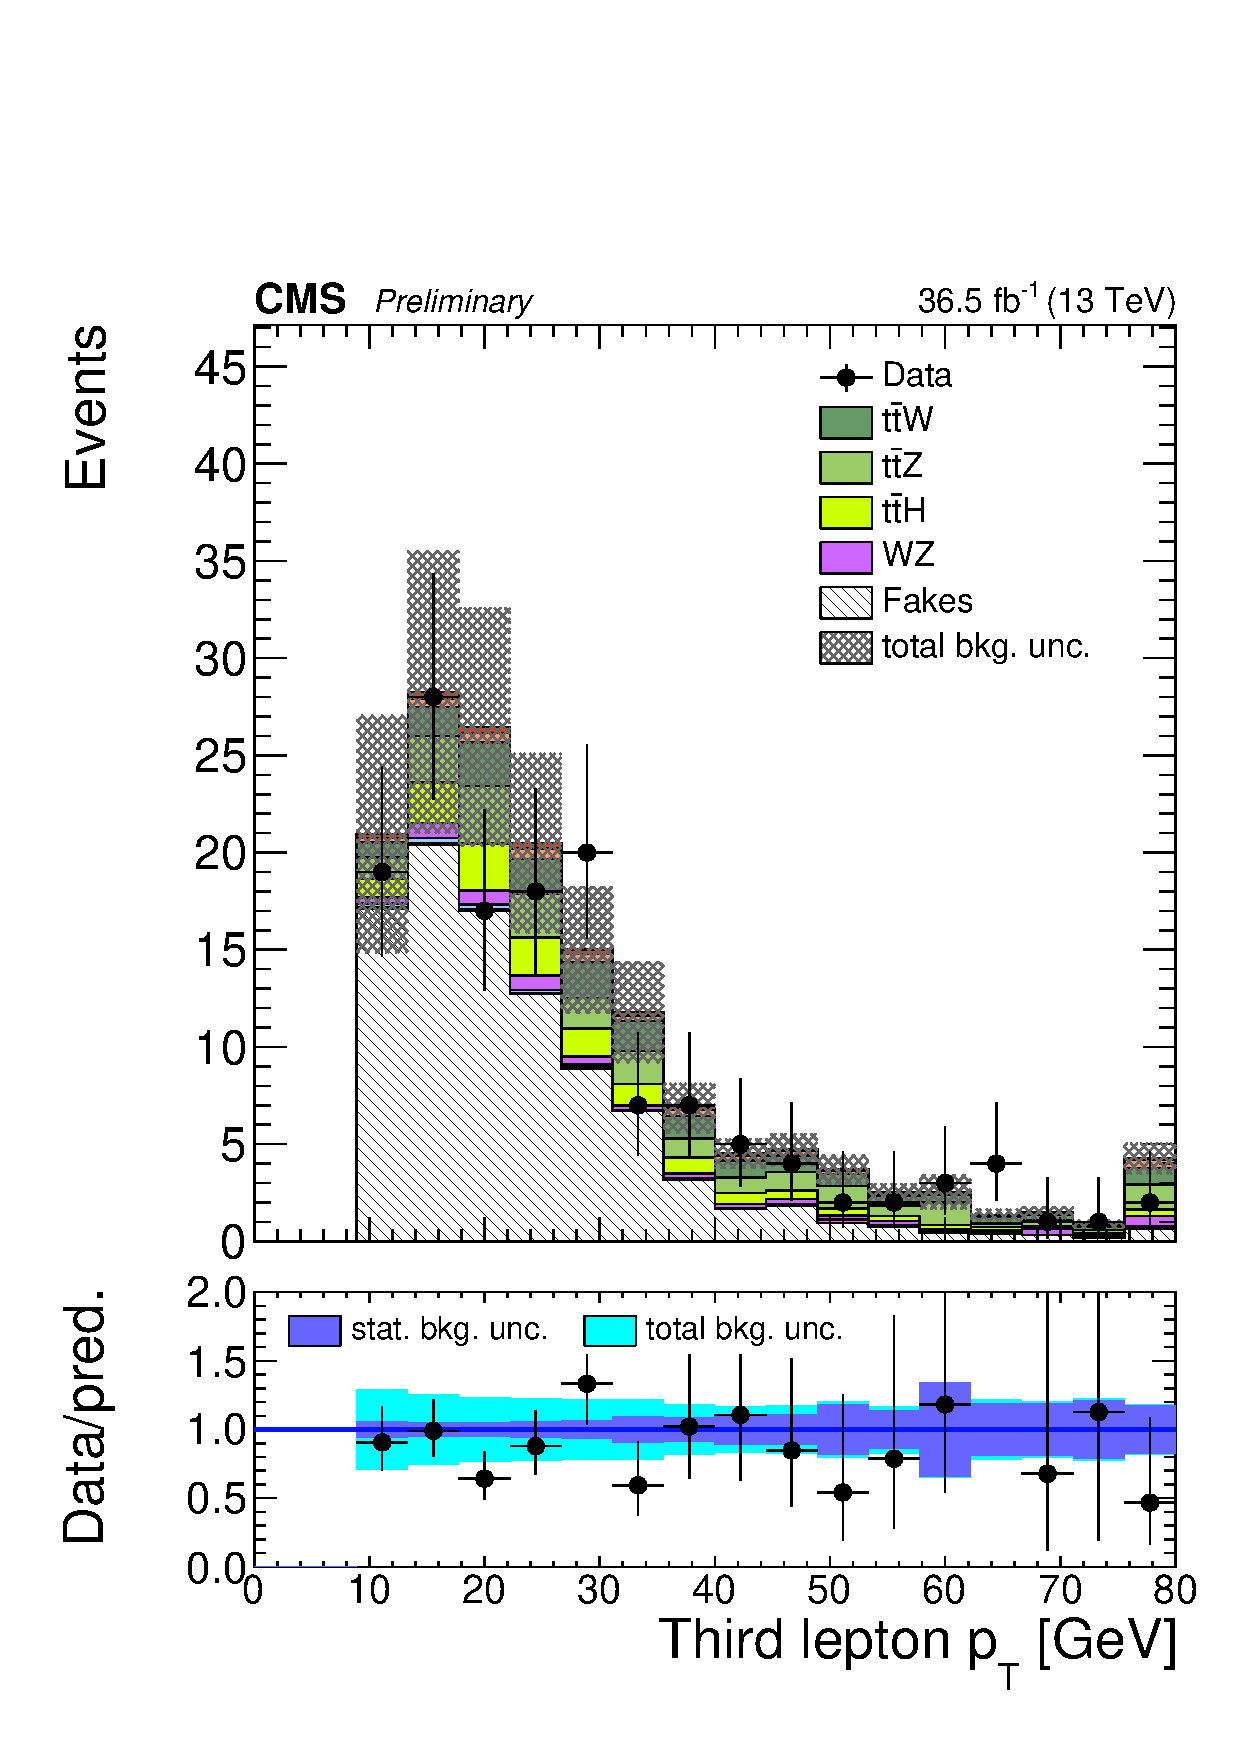
\includegraphics[width=0.28\textwidth]{3lsignal/Lep3Pt.pdf}
  \includegraphics[width=0.28\textwidth]{3lsignal/dEtaFwdJetBJet_40.pdf}
  \includegraphics[width=0.28\textwidth]{3lsignal/dEtaFwdJet2BJet_40.pdf}\\
  \includegraphics[width=0.28\textwidth]{3lsignal/dEtaFwdJetClosestLep_40.pdf}
  \includegraphics[width=0.28\textwidth]{3lsignal/dPhiHighestPtSSPair.pdf}
  \includegraphics[width=0.28\textwidth]{3lsignal/maxEtaJet25_40.pdf}\\
  \includegraphics[width=0.28\textwidth]{3lsignal/minDRll.pdf}
  \includegraphics[width=0.28\textwidth]{3lsignal/nJet25.pdf}
  \includegraphics[width=0.28\textwidth]{3lsignal/nJetEta1_40.pdf}\\
  \includegraphics[width=0.28\textwidth]{3lsignal/totCharge.pdf}
  \caption{Distributions of input variables to the BDT for signal discrimination, three lepton channel, normalized to their cross section and to 35.9\fbinv.}
  \label{fig:input_vars_3l_xsec}
\end{figure}

\begin{figure} [!h]
  \centering
  \includegraphics[width=0.22\textwidth]{signalregion_2lss/mumu/Lep2Pt.pdf}
  \includegraphics[width=0.22\textwidth]{signalregion_2lss/mumu/dEtaFwdJetBJet_40.pdf}
  \includegraphics[width=0.22\textwidth]{signalregion_2lss/mumu/dEtaFwdJet2BJet_40.pdf}
  \includegraphics[width=0.22\textwidth]{signalregion_2lss/mumu/dEtaFwdJetClosestLep_40.pdf} \\
  \includegraphics[width=0.22\textwidth]{signalregion_2lss/mumu/dPhiHighestPtSSPair.pdf}
  \includegraphics[width=0.22\textwidth]{signalregion_2lss/mumu/maxEtaJet25_40.pdf}
  \includegraphics[width=0.22\textwidth]{signalregion_2lss/mumu/minDRll.pdf}
  \includegraphics[width=0.22\textwidth]{signalregion_2lss/mumu/nJet25.pdf} \\
  \includegraphics[width=0.22\textwidth]{signalregion_2lss/mumu/nJetEta1_40.pdf}
  \includegraphics[width=0.22\textwidth]{signalregion_2lss/mumu/totCharge.pdf}
  \caption{Distributions of input variables to the BDT for signal discrimination, in \mumu\ channel, normalized to their cross section and to 35.9\fbinv.}
  \label{fig:input_vars_2lss_xsec_mumu}
\end{figure}

\begin{figure} [!h]
  \centering
  \includegraphics[width=0.22\textwidth]{signalregion_2lss/emu/Lep2Pt.pdf}
  \includegraphics[width=0.22\textwidth]{signalregion_2lss/emu/dEtaFwdJetBJet_40.pdf}
  \includegraphics[width=0.22\textwidth]{signalregion_2lss/emu/dEtaFwdJet2BJet_40.pdf}
  \includegraphics[width=0.22\textwidth]{signalregion_2lss/emu/dEtaFwdJetClosestLep_40.pdf} \\
  \includegraphics[width=0.22\textwidth]{signalregion_2lss/emu/dPhiHighestPtSSPair.pdf}
  \includegraphics[width=0.22\textwidth]{signalregion_2lss/emu/maxEtaJet25_40.pdf}
  \includegraphics[width=0.22\textwidth]{signalregion_2lss/emu/minDRll.pdf}
  \includegraphics[width=0.22\textwidth]{signalregion_2lss/emu/nJet25.pdf} \\
  \includegraphics[width=0.22\textwidth]{signalregion_2lss/emu/nJetEta1_40.pdf}
  \includegraphics[width=0.22\textwidth]{signalregion_2lss/emu/totCharge.pdf}
  \caption{Distributions of input variables to the BDT for signal discrimination, in $\emu$ channel, normalized to their cross section and to 35.9\fbinv.}
  \label{fig:input_vars_2lss_xsec_emu}
\end{figure}
%% \begin{figure} [!h]
%%   \centering
%%   \includegraphics[width=0.22\textwidth]{signalregion_2lss/ee/Lep2Pt.pdf}
%%   \includegraphics[width=0.22\textwidth]{signalregion_2lss/ee/dEtaFwdJetBJet_40.pdf}
%%   \includegraphics[width=0.22\textwidth]{signalregion_2lss/ee/dEtaFwdJet2BJet_40.pdf}
%%   \includegraphics[width=0.22\textwidth]{signalregion_2lss/ee/dEtaFwdJetClosestLep_40.pdf} \\
%%   \includegraphics[width=0.22\textwidth]{signalregion_2lss/ee/dPhiHighestPtSSPair.pdf}
%%   \includegraphics[width=0.22\textwidth]{signalregion_2lss/ee/maxEtaJet25_40.pdf}
%%   \includegraphics[width=0.22\textwidth]{signalregion_2lss/ee/minDRll.pdf}
%%   \includegraphics[width=0.22\textwidth]{signalregion_2lss/ee/nJet25.pdf} \\
%%   \includegraphics[width=0.22\textwidth]{signalregion_2lss/ee/nJetEta1_40.pdf}
%%   \includegraphics[width=0.22\textwidth]{signalregion_2lss/ee/totCharge.pdf}
%%   \caption{Distributions of input variables to the BDT for signal discrimination, in $\ee$ channel, normalized to their cross section and to 35.9\fbinv.}
%%   \label{fig:input_vars_2lss_xsec_ee}
%% \end{figure}

